\documentclass[tikz, border=10pt]{standalone}

% --- Essential packages for figures and drawing ---
\usepackage[utf8]{inputenc}
\usepackage{tikz}
\usetikzlibrary{calc, shapes.geometric, positioning}

% --- Define custom colors ---
\definecolor{sourcecolor}{RGB}{204, 0, 0}   % Red for Source
\definecolor{targetcolor}{RGB}{0, 102, 204} % Blue for Target
\definecolor{matchcolor}{RGB}{0, 153, 76}   % Green for matches/math

\begin{document}

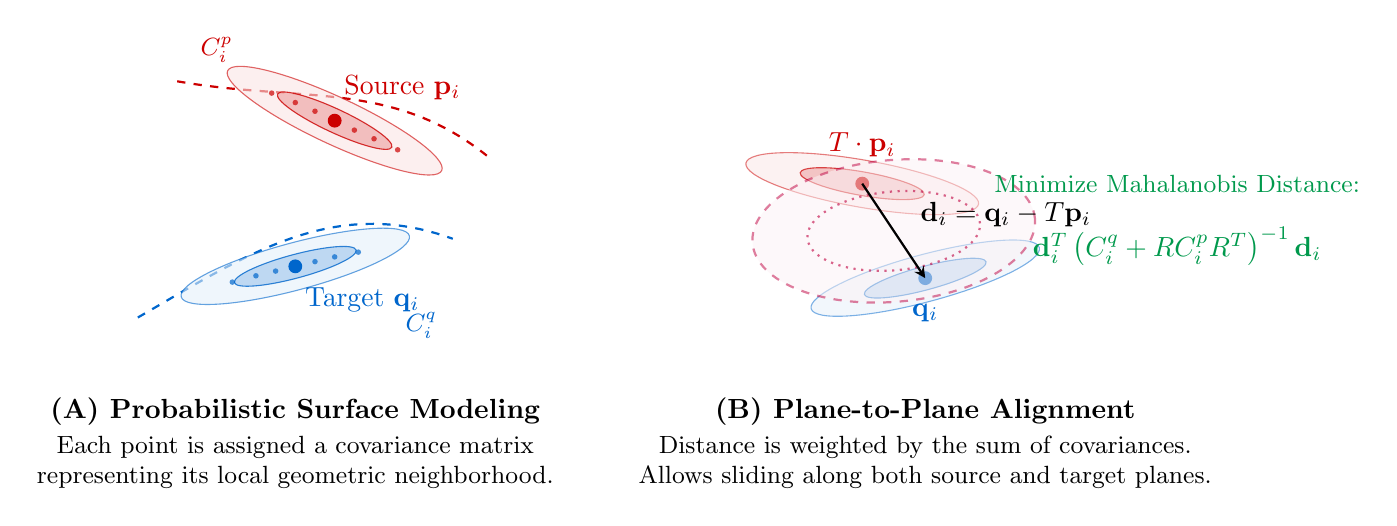
\begin{tikzpicture}[scale=1.0, >=stealth]

    % ==========================================
    % --- Figure (A): Local Covariance Modeling ---
    % ==========================================
    \begin{scope}[shift={(0,0)}]
        
        % Target Surface (Blue)
        \draw[targetcolor, thick, dashed] (0, 0.5) to[out=30, in=160] (4, 1.5);
        \coordinate (Q) at (2, 1.15); % A point on the target surface
        
        % Target Covariance Ellipses (Concentric for probability density)
        \draw[targetcolor, fill=targetcolor!10, opacity=0.6] (Q) [rotate around={15:(Q)}] ellipse (1.5 and 0.3);
        \draw[targetcolor, fill=targetcolor!30, opacity=0.8] (Q) [rotate around={15:(Q)}] ellipse (0.8 and 0.15);
        
        % Neighborhood point cloud (Target)
        \foreach \x/\y in {1.2/0.95, 1.5/1.03, 1.75/1.09, 2.25/1.21, 2.5/1.27, 2.8/1.33}
            \fill[targetcolor, opacity=0.7] (\x,\y) circle (1pt);

        % Target Point and Label
        \fill[targetcolor] (Q) circle (2.5pt) node[below right, yshift=-4pt] {Target $\mathbf{q}_i$};
        \node[targetcolor, font=\small] at (3.6, 0.4) {$C_i^q$};

        % Source Surface (Red)
        \draw[sourcecolor, thick, dashed] (0.5, 3.5) to[out=-10, in=140] (4.5, 2.5);
        \coordinate (P) at (2.5, 3.0); % A point on the source surface
        
        % Source Covariance Ellipses (Concentric for probability density)
        \draw[sourcecolor, fill=sourcecolor!10, opacity=0.6] (P) [rotate around={-25:(P)}] ellipse (1.5 and 0.3);
        \draw[sourcecolor, fill=sourcecolor!30, opacity=0.8] (P) [rotate around={-25:(P)}] ellipse (0.8 and 0.15);
        
        % Neighborhood point cloud (Source)
        \foreach \x/\y in {1.7/3.35, 2.0/3.23, 2.25/3.12, 2.75/2.88, 3.0/2.77, 3.3/2.63}
            \fill[sourcecolor, opacity=0.7] (\x,\y) circle (1pt);

        % Source Point and Label
        \fill[sourcecolor] (P) circle (2.5pt) node[above right, yshift=4pt] {Source $\mathbf{p}_i$};
        \node[sourcecolor, font=\small] at (1.0, 3.9) {$C_i^p$};

        % Labels
        \node[anchor=south, font=\bfseries] at (2, -1) {(A) Probabilistic Surface Modeling};
        \node[anchor=south, font=\small, align=center] at (2, -1.8) {Each point is assigned a covariance matrix\\representing its local geometric neighborhood.};
        
    \end{scope}

    % ==========================================
    % --- Figure (B): G-ICP Plane-to-Plane Matching ---
    % ==========================================
    \begin{scope}[shift={(8,0)}]
        
        % Target Point & Covariance
        \coordinate (Q2) at (2, 1);
        \draw[targetcolor, fill=targetcolor!10, opacity=0.5] (Q2) [rotate around={15:(Q2)}] ellipse (1.5 and 0.3);
        \draw[targetcolor, fill=targetcolor!30, opacity=0.7] (Q2) [rotate around={15:(Q2)}] ellipse (0.8 and 0.15);
        \fill[targetcolor] (Q2) circle (2.5pt) node[below=6pt] {$\mathbf{q}_i$};

        % Transformed Source Point & Covariance
        \coordinate (P2) at (1.2, 2.2);
        \draw[sourcecolor, fill=sourcecolor!10, opacity=0.5] (P2) [rotate around={-10:(P2)}] ellipse (1.5 and 0.3);
        \draw[sourcecolor, fill=sourcecolor!30, opacity=0.7] (P2) [rotate around={-10:(P2)}] ellipse (0.8 and 0.15);
        \fill[sourcecolor] (P2) circle (2.5pt) node[above=6pt] {$T \cdot \mathbf{p}_i$};

        % Combined Covariance (Conceptually minimized)
        % Multi-layered to show probability distribution
        \draw[purple, dashed, thick, fill=purple!5, opacity=0.5] (1.6, 1.6) [rotate around={5:(1.6,1.6)}] ellipse (1.8 and 0.9);
        \draw[purple, dotted, thick, opacity=0.6] (1.6, 1.6) [rotate around={5:(1.6,1.6)}] ellipse (1.1 and 0.5);

        % Distance Vector
        \draw[thick, ->, black] (P2) -- (Q2) node[midway, right, xshift=6pt, yshift=6pt] {$\mathbf{d}_i = \mathbf{q}_i - T \mathbf{p}_i$};

        % Formula annotation (Shifted right to avoid overlapping the ellipses)
        \node[matchcolor, font=\small, align=left] at (5.2, 2.2) {Minimize Mahalanobis Distance:};
        \node[matchcolor, font=\normalsize] at (5.2, 1.4) {$\mathbf{d}_i^T \left( C_i^q + R C_i^p R^T \right)^{-1} \mathbf{d}_i$};

        % Labels
        \node[anchor=south, font=\bfseries] at (2, -1) {(B) Plane-to-Plane Alignment};
        \node[anchor=south, font=\small, align=center] at (2, -1.8) {Distance is weighted by the sum of covariances.\\Allows sliding along both source and target planes.};

    \end{scope}

\end{tikzpicture}

\end{document}